% Sample LaTeX file for creating a paper in the Morgan Kaufmannn two
% column, 8 1/2 by 11 inch proceedings format.

\documentclass{article}

\usepackage{proceed2e}

% use Times
%\usepackage{times}
% For figures
\usepackage{graphicx} % more modern
%\usepackage{epsfig} % less modern
\usepackage{subfigure} 

% For citations
\usepackage{natbib}

\usepackage{url}
% For algorithms
\usepackage{algorithm}
\usepackage{algorithmic}

\usepackage{amsmath,amssymb} 
\usepackage{makecell}
\usepackage{booktabs}

\usepackage{helvet}
\usepackage{courier}

\usepackage{hyperref}


\newtheorem{theorem}{Theorem}[section]
\newtheorem{lemma}[theorem]{Lemma}
\newtheorem{proposition}[theorem]{Proposition}
\newtheorem{corollary}[theorem]{Corollary}
\newcommand{\shortcite}[1]{\cite{#1}}

\newcommand{\argmax}{\mathop\mathrm{argmax}}
\newcommand{\argmin}{\mathop\mathrm{argmin}}

\newenvironment{proof}[1][Proof]{\begin{trivlist}
\item[\hskip \labelsep {\bfseries #1}]}{\end{trivlist}}
\newenvironment{definition}[1][Definition]{\begin{trivlist}
\item[\hskip \labelsep {\bfseries #1}]}{\end{trivlist}}
\newenvironment{example}[1][Example]{\begin{trivlist}
\item[\hskip \labelsep {\bfseries #1}]}{\end{trivlist}}
\newenvironment{remark}[1][Remark]{\begin{trivlist}
\item[\hskip \labelsep {\bfseries #1}]}{\end{trivlist}}
\newcommand{\qed}{\nobreak \ifvmode \relax \else
      \ifdim\lastskip<1.5em \hskip-\lastskip
      \hskip1.5em plus0em minus0.5em \fi \nobreak
      \vrule height0.75em width0.5em depth0.25em\fi}

\newcommand{\notejp}[1]{\textcolor{red}{JP: #1}}


% Packages hyperref and algorithmic misbehave sometimes.  We can fix
% this with the following command.
\newcommand{\theHalgorithm}{\arabic{algorithm}}



\title{Stochastic Optimization of Black-box Functions on Riemannian Manifolds Using Kernel Adaptive Sequential Monte Carlo}

\author{} % LEAVE BLANK FOR ORIGINAL SUBMISSION.
          % UAI  reviewing is double-blind.

% The author names and affiliations should appear only in the accepted paper.
%
%\author{ {\bf Harry Q.~Bovik\thanks{Footnote for author to give an
%alternate address.}} \\
%Computer Science Dept. \\
%Cranberry University\\
%Pittsburgh, PA 15213 \\
%\And
%{\bf Coauthor}  \\
%Affiliation          \\
%Address \\
%\And
%{\bf Coauthor}   \\
%Affiliation \\
%Address    \\
%(if needed)\\
%}

\begin{document}

\maketitle

\begin{abstract}
This paper puts forward a new stochastic method for global optimization of black-box functions on a Riemannien manifold $\mathcal{M}$,   
which is rather challenging yet useful in many areas. The proposed algorithm is based on \emph{Kernel Adaptive Sequential 
Monte Carlo} (KASMC) by exploiting the closeness between simulated annealing and sequential Monte Carlo (SMC), and thus is referred to as KASMC optimizer.             
At each Markov chain Monte Carlo (MCMC) transition of KASMC optimizer, samples are first proposed in a reproducing kernel Hilbert space (RKHS) of the ``envelop space" 
of $\mathcal{M}$, after tempered acceptance criterion, then they are mapped back to the envelop space and $\mathcal{M}$ respectively by two projection steps.     
The strength of KASMC optimizer, compared to classical simulated annealing, stems from its two adaptive  
tunning mechanisms. The first one is adaptive tempering, which automatically constructs temperature schedule through cooling; 
the second one is adaptive MCMC transition in RKHS, which is 
critical to handle nonlinearity of support of functions on $\mathcal{M}$. Results in our experiments demonstrates the 
promising applicability of KASMC optimizer. 
\end{abstract}

\section{Introduction}
Global optimization on a black-box function $f$ has been a challenging task  
despite its wide usage in many disciplines \citep{black_box_optimization, black_box_optimization_book}.    
Difficulties are usually considered from two aspects: \emph{i}. the analytic form of $f$ is unknown and function values can 
be only accessed point-wisely, thus no function landscape property (e.g. convexity) can be exploited for numerical solutions;     
\emph{ii}. function evaluation at one point is usually at high cost, which narrows algorithms to be practical only if it can find 
optimal (or with tolerant imprecision) with an affordable iteration budget. In this paper, we consider an even more ``nasty" case, where 
$f$ is defined on a Riemannien manifold $\mathcal{M}$. Since the support of $f$ is $\mathcal{M}$ instead of $\mathbb{R}^d$, search     
is supposed to be more careful since exploration and exploitation is restricted to $\mathcal{M}$.       
Very often the shape of $\mathcal{M}$ is irregular, which worsens the situation.       
However, this task arises in many areas \citep{SA_registration, Geo_MCMC}, 
\emph{e.g.} rotation optimization to find best shape registration, simplex optimization to best fit categorical 
distributions. Therefore, it is rather desirable to come up with a general algorithm which can efficiently find good solutions with guaranteed precision. 

\emph{Simulated annealing} (SA) is a classical stochastic optimization for black-box functions \citep{SA}. However, its applicability is limited to common case where $f$ is 
defined on $\mathbb{R}^d$. 
In present paper, we propose a novel stochastic method to extend simulated annealing to handle $f$ on Remannian manifolds. 
The proposed algorithm is based on \emph{Kernel Adaptive Sequential Monte Carlo}     
(KASMC) by exploiting the close relation between SA and sequential Monte Carlo (SMC), and therefore is referred to as KASCM optimizer.    
Similar to SA, KASMC optimizer increases the determinism of proposal acceptance criterion by monotonically decreasing a temperature parameter.     
However, in KASMC, sequential tempering is implemented in a SMC instead, which can be considered as a multi-particle simulated annealing \citep{multi_particle} 
with weighting and resampling.      
At each Markov chain Monte Carlo (MCMC) transition in the SMC, samples are first proposed in a reproducing kernel Hilbert space (RKHS) of the ``envelop space" 
of $\mathcal{M}$, after tempered acceptance criterion, then they are mapped back to the envelop space and $\mathcal{M}$ respectively by two projection steps.     
The adaptive proposal construction in RKHS is inspired by MCMC Kameleon \citep{MCMC_Kameleon}. 
The strength of KASMC optimizer stems from its two adaptive  
tunning mechanisms. The first one is adaptive tempering, which, based on \emph{effective sampling size} (ESS), automatically constructs temperature schedule 
through cooling; 
the second one is adaptive MCMC transition in RKHS, which is 
critical to handle nonlinearity of support of $f$ on $\mathcal{M}$. 
Based on previous study, which includes the finite-time performance guarantees of simulated annealing on continuous domains \citep{SA_finite_time}         
and convergence property of adaptive SMC \citep{convergence_ASMC}, KASMC optimizer is expected to work efficiently and effectively.   
In our experiments, the proposed KASMC optimizer was evaluated on a practical task: optimal rotation search for 3D registration.  
Two Riemannian manifolds were tried: unit quaternion manifold and $SO(3)$ manifold. According to our empirical results, KASMC optimizer consistently 
outperforms SA and other non-adaptive counterparts.   

This paper makes four contributions.  First, we reveal the closeness between SA and SMC, which sheds light on new insights into these two techniques.
Second, to better fit nonlinear support (here Riemannian manifold), MCMC Kameleon is for the first time employed in adaptive SMC.          
Third, we put forward a simpler yet better pre-image method to replace the naive one-step gradient projection in MCMC Kameleon.       
Last but not least, a stochastic optimization method of black-box functions on Riemannian manifolds is proposed. Under some weak assumptions, it can be widely applied 
on general functions and Riemannian manifolds. 


\subsection{Related Work}
KASMC optimizer can be related to many other work from different perspectives. The following provides a short summary of recent development of relevant study. 
\paragraph{Black-box function global optimization.} A review of historical methods for black-box function global optimization can be found in 
\cite{black_box_optimization} or \cite{black_box_optimization_book}.   
Out of all work, \emph{Bayesian optimization} \citep{BO_tutorial,BO_NIPS} 
and \emph{Hierarchical optimistic optimization} \citep{optimistic}
are two particularly notable research branches which have recently attracted particularly more attention.  
Bayesian optimization is an extension \emph{response surface method} with Gaussian process to interpolate  
the unknown function $f$. Hierarchical optimistic optimization is an application of \emph{optimism principle} on 
\emph{Monte Carlo tree search} (MCTS), which partitions search spaces hierarchical and conducts exploration and 
exploitation at different scales. A combination of these two techniques was proposed in \cite{Bam_SOO}. 
To the best of our knowledge, no work has been conducted for Bayesian optimization or optimistic optimization on Riemannian 
manifolds. Only one work on Bayesian optimization with constraints \citep{BO_constraint} can be extended to Reimannian manifolds.        

\paragraph{SA and SMC.} On the one hand, SA is a stochastic optimization and it was originally proposed as an adaption of Metropolis-Hasting algorithm to obtain samples 
from thermodynamic systems \citep{SA}.  On the other hand, SMC is sampler for state-space models or complex distributions \citep{SMC}. 
Since SMC is more often used in filtering 
community, it is also referred to as \emph{particle filter} and also its samples are called particles.  
Although two methods are motivated for different purposes,  

\paragraph{Adaptive SMC}
\citep{SMC_ABC, ASMC_1, ASMC_binary}, 
\paragraph{MCMC on Riemannian Manifold}




\section{Preliminaries}
\subsection{Assumptions}

First level headings are all caps, flush left, bold and in point size
12. One line space before the first level heading and 1/2~line space
after the first level heading.

\subsection{Simulated Annealing}

Second level headings must be flush left, all caps, bold and in point
size 10. One line space before the second level heading and 1/2~line
space after the second level heading.

\subsection{Sequential Monte Carlo Sampler}

Third level headings must be flush left, initial caps, bold, and in
point size 10.  One line space before the third level heading and
1/2~line space after the third level heading.

\subsection{Adaptive Tempering}


\subsection{Kernel Adaptive MCMC}


\subsection{Optimization on Riemannian Manifolds}



\section{Proposed Algorithm}

\subsection{Overview}
\begin{figure*}[t]
	\centering
	\includegraphics[width=0.85\textwidth]{overview}
	\caption{An overview of kernel Adaptive MCMC transition and two inverse projection steps.}
	\label{fig:over_view}
\end{figure*}

\subsection{Pre-Image}

\begin{figure}[t]
	\centering
	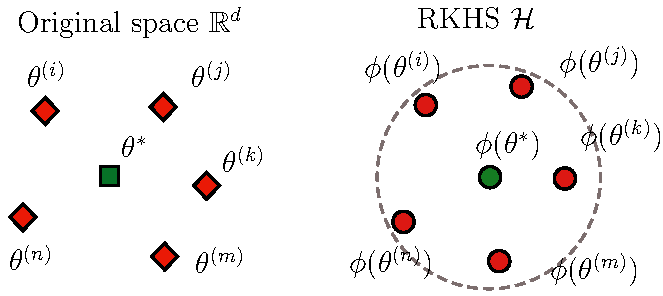
\includegraphics[width=0.5\textwidth]{pre-image}
	\caption{Pre-image by using local topology consistence.  }
	\label{fig:over_view}
\end{figure}


\subsection{Projection onto $\mathcal{M}$}

\section{Experiments}
\subsection{Unit Quaternion Manifold Optimization}
\subsection{SO(3) Manifold Optimization}

%\subsubsection*{Acknowledgements}
%Use unnumbered third level headings for the acknowledgements title.
%All acknowledgements go at the end of the paper.


\bibliographystyle{plainnat}
\bibliography{refs}

\end{document}
